\documentclass[fleqn]{article}

\usepackage[utf8]{inputenc}
\usepackage{fullpage}
\usepackage{graphicx}
\usepackage{amsmath}
\usepackage{amsmath,amssymb}
\usepackage{mathbbol}
\usepackage{chngcntr}
\usepackage{hyperref}
\DeclareMathOperator{\E}{\mathbb{E}}
\DeclareMathOperator{\V}{\mathbb{Var}}
\DeclareMathOperator{\B}{\mathbb{Bias}}
\counterwithin*{equation}{subsection}
\counterwithin*{equation}{section}

\begin{document}

\section*{Problem 3.2}

So we first need to prove that matrix $\Psi = \Phi(\Phi^\top\Phi)^{-1}\Phi^\top$ projects any N-dimensional vector $v$ onto the subspace spanned by M columns of $\Phi$ (lets denote this subspace as $S(\Phi)$). Here we just assume $(\Phi^\top\Phi)^{-1}$ exists (i.e. $\Phi^\top\Phi$ is invertible) since it is a part of the definition of the matrix given in the problem condition.

Let us consider any N-dimensional vector $v$. We need to prove that there exist $\alpha_1\ldots\alpha_M \in \mathbb{R}$ such that $\Psi v = \alpha_1\varphi_1(D) + \ldots + \alpha_M\varphi_M(D)$. If we denote $\alpha = (\alpha_1,\ldots,\alpha_M)^\top$, then we need to prove there exists M-dimensional vector $\alpha$ such that $\Phi\cdot\alpha = \Psi v$. We notice now that $\alpha = (\Phi^\top\Phi)^{-1}\Phi^\top v$ is the very vector we are looking for, so it exists, so we proved that $\Psi$ indeed projects $v$ onto the subspace of columns of $\Phi$. 

Lets us now consider $w_{ML} = (\Phi^\top\Phi)^{-1}\Phi^\top t$. We need to prove $y = \Phi w_{ML}$ is an orthogonal projection of $t$ onto the subspace of columns of $\Phi$. This means, we need to prove $ y - t \hspace*{0.05in} \bot \hspace*{0.05in} S(\Phi) $. This is the same as proving that $\Phi(\Phi^\top\Phi)^{-1}\Phi^\top t - t \bot S(\Phi)$.

Consider left part of the statement and multiply it by $\Phi^\top$. This gives us  $\Phi^\top (\Phi(\Phi^\top\Phi)^{-1}\Phi^\top t - t) = (\Phi^\top\Phi)(\Phi^\top\Phi)^{-1}\Phi^\top t - \Phi^\top t = \mathbb{0}$. So, we see that all the columns of $\Phi$ are orthogonal with $\Phi(\Phi^\top\Phi)^{-1}\Phi^\top t - t$, which means $\Phi(\Phi^\top\Phi)^{-1}\Phi^\top t$ is an orthogonal projection of $t$ onto $S(\Phi)$.

\section*{Problem 3.3}

Since $w^*$ is extremum, we can equate $E_D$ gradient to zero:
\begin{align}
\nabla E_D = -\sum\limits_{n=1}^Nr_n(t_n - w^\top\varphi(x_n))\varphi^\top(x_n) = 0 
\label{eq:defxyz}
\end{align}

Let us consider $R = \begin{pmatrix}
r_1 & 0 & ... & 0 \\
0 & r_2 & ... & 0 \\
0 & 0 & ... & 0 \\
0 & 0 & ... & r_n
\end{pmatrix}$

We can rewrite equation $\ref{eq:defxyz}$ in the following way:

\begin{align}
\nabla E_D = -\Phi^\top R t + \Phi^\top R \Phi w = 0
\end{align}

Thus we obtain 

\begin{align}
w^* = (\Phi^\top R \Phi) ^{-1}\Phi^\top R t
\end{align}

We can consider the matrix R, one the one hand, as inverse data-dependent noise variance: different $x_i$ will have different correspondent $r_i$, and the smaller $r_i$ is, the smaller is the impact of $i_{th}$ sample. So, $r_i$ can be used as our confidence in the $t_i$ value.

On the other hand, at least when $r_i$ is integer, it can be considered as the number of times sample $(x_i, t_i)$ was present in the dataset.



\section*{Problem 3.4}

Let us average error function over all possible noise values, i.e. let us compute it's expected value with respect to added noise $\{\epsilon_i\}$. Lets us denote $x_n' = x_n + \epsilon_n$ - input variable with added noise.

\begin{align}
\E[E_D] & = \E[\frac{1}{2}\sum\limits_{n=1}^N\{y(x_n',w) - t_n\}^2] = \\ & = \E[\frac{1}{2}\sum\limits_{n=1}^N\{w_0 + \sum\limits_{i=1}^D w_i (x_{ni} + \epsilon_{ni}) - t_n\}^2 = \\ & = \E[\frac{1}{2}\sum\limits_{n=1}^N\{w_0 + \sum\limits_{i=1}^D w_i (x_{ni} + \epsilon_{ni}) - t_n\} = \\ & = \frac{1}{2}\sum\limits_{n=1}^N\E[\{w_0 -t_n + \sum\limits_{i=1}^D w_i (x_{ni} + \epsilon_{ni}) \}^2] = \\
& = \frac{1}{2}\sum\limits_{n=1}^N\E[(w_0-t_n)^2 + (w_0-t_n)\sum\limits_{i=1}^D w_i(x_{ni}+\epsilon_{ni}) + \sum\limits_{i,j=1}^Dw_iw_j(x_{ni}+\epsilon_{ni})(x_{nj}+\epsilon_{nj})] = \\ & = \frac{1}{2}\sum\limits_{n=1}^N\{(w_0-t_n)^2 + (w_0-t_n)\sum\limits_{i=1}^D w_ix_{ni} + \sum\limits_{i,j=1}^Dw_iw_j(x_{ni}x_{nj} + \delta_{ij}\sigma^2) \} = \\
& = \frac{1}{2}\sum\limits_{n=1}^N\{y(x_n,w) - t_n\}^2 + \frac{N \sigma^2}{2}w^\top w
\end{align}


So, as expected, we see that error function, averaged over noise values, gives us weight-decayed sum-of-squares error function over noise-free input variables with omitted bias in regularization term, so minimizing the latter gives the same result as minimizing the former.  

\section*{Problem 3.5}

Suppose we want to minimize $E_D(w)$ subject to $\sum\limits_{j=1}^M|w_j|^q \le \eta$
This is equivalent to minimizing Lagrange function $L(w, \lambda) = E_D(w) + \lambda'(\sum\limits_{j=1}^M(|w_j|^q - \eta)$ under conditions that $\lambda' \ge 0$, $\sum\limits_{j=1}^M|w_j|^q \le \eta$ and $\lambda'(\sum\limits_{j=1}^M|w_j|^q - \eta) = 0$. When we use regularization, we suppose we only vary $\{w_j\}$ while keeping $\lambda$ fixed. So we can substitute $\lambda' = \frac{\lambda}{2}$ and pay no attention to $\eta$ since it is constant, and try to minimize the Lagrangian which now takes form of $E_D(w) + \frac{\lambda}{2}(\sum\limits_{j=1}^M(|w_j|^q)$, and this is exactly the regularized least squares error function. 

To find the dependence between $\eta$ and $w$ we note that for optimal solution $\{w_j^*\}$ we have $\eta = \sum\limits_{j=1}^M(|w_j^*|^q)$.

As of dependence between $\eta$ and $\lambda$ we can see that the greater $\lambda$ is, the more is regularization effect and so the less will be $\eta$. 

\section*{Problem 3.6}

This problem looks simple, but in fact to understand it deeply one need to perform certain actions. First of all, we will write down the log-likelihood of the dataset with given W:

\begin{align}
L(D) = \prod\limits_{n=1}^N (2\pi)^-{\frac{k}{2}}|\Sigma|^{-\frac{1}{2}}\exp(-\frac{1}{2}(t_n - W^\top\varphi(X_n))^\top\Sigma^{-1}(t_n - W^\top\varphi(X_n))
\end{align}

\begin{align}
\log L(D) = -\frac{kN}{2}\log(2\pi) -\frac{N}{2}|\Sigma| - \frac{1}{2} \sum\limits_{n=1}^N(t_n - W^\top\varphi(X_n))^\top\Sigma^{-1}(t_n - W^\top\varphi(X_n))
\end{align}

We now want to find the maximum of the log-likelihood with respect to W to find $W_{ML}$. To achieve this, we will use matrix derivatives notation (see \url{https://en.wikipedia.org/wiki/Matrix_calculus})

In fact, we see that taking derivative of scalar with respect to matrix gives us a matrix of the same size:

$\frac{\partial \log L(D)}{\partial W} = \begin{pmatrix}
\frac{\partial \log L(D)}{\partial W_{11}} & \frac{\partial \log L(D)}{\partial W_{12}} & ... & \frac{\partial \log L(D)}{\partial W_{1K}} \\
\frac{\partial \log L(D)}{\partial W_{21}} & \frac{\partial \log L(D)}{\partial W_{22}} & ... & \frac{\partial \log L(D)}{\partial W_{2K}} \\
... & ... & ... & ... \\
\frac{\partial \log L(D)}{\partial W_{M1}} & \frac{\partial \log L(D)}{\partial W_{M2}} & ... & \frac{\partial \log L(D)}{\partial W_{MK}}
\end{pmatrix}$


To get the work done, we first prove following identity:

\begin{align}
\frac{\partial (Xa + b)^\top C (Xa + b)}{\partial X} = (C + C^\top)(Xa + b)a^\top
\end{align}

Here, $C$ is a square matrix of some size $N \times N$, $b$ is a vector of size $N$, $a$ is a vector of size $M$, and $X$ is $M \times N$ matrix.  

To prove it, let's use write down the numerator in non-matrix form:

\begin{align}
(Xa + b)^\top C (Xa + b) = \sum\limits_{l=1}^N(\sum\limits_{k=1}^N(\sum\limits_{\beta=1}^MX_{l\beta}a_\beta + b_l)C_{kl})(\sum\limits_{\gamma=1}^NX_{k\gamma}a_\gamma + b_k)
\end{align}

Taking now derivative of this with respect to $X_{ij}$ we get:

\begin{align}
\frac{\partial (Xa + b)^\top C (Xa + b)}{\partial X_{ij}} &= \sum\limits_{k=1}^Na_jC_{ki} (X_ka + b_k) + \sum\limits_{l=1}^N(X_la + b_l)C_{il}a_j = \\ & = a_j[{C^i}^\top(Xa + b) + (Xa + b)^\top C_i] =\\ & = (C + C^\top)_i(Xa + b)a_j
\end{align}

So, we see that $\frac{\partial (Xa + b)^\top C (Xa + b)}{\partial X} = (C + C^\top)(Xa + b)a^\top$.

Now, returning to the original problem, we have 

\begin{align}\frac{\partial \log L(D)}{\partial W} & = -\frac{1}{2}\sum\limits_{n=1}^N(\Sigma^{-1} + {\Sigma^{-1}}^{\top})(t_n - W^\top \varphi(X_n))\varphi(X_n)^\top = \\ & = \Sigma^{-1} (T^\top - W^\top \varPhi^\top)\varPhi = 0
\end{align}

Just a reminder, $T$ is a $N \times K$ matrix, $\varPhi(X)$ is a $N \times M$ matrix, and $W$ is $M \times K$ matrix. 

So assigning this to 0 and reducing $\Sigma^{-1}$ we get $T^\top \varPhi = W_{ML}^\top \varPhi^\top \varPhi$ and so $W_{ML} =  (\varPhi^\top \varPhi)^{-1}\varPhi^\top T$ which shows us that indeed $i$-th column of $W_{ML}$ has the same well known form of $W_{ML_i}=(\varPhi^\top \varPhi)^{-1}\varPhi^\top t_i$ and $W_{ML}$ is independent of $\Sigma$.

Now let us consider 

\begin{align}\frac{\partial \log L(D)}{\partial \Sigma^{-1}} & = -\frac{N}{2}\frac{\partial\log|\Sigma|}{\partial\Sigma^{-1}} - \frac{1}{2}\sum\limits_{n=1}^N(t_n - W_{ML}^\top \varphi(X_n))(t_n - W_{ML}^\top \varphi(X_n))^\top = \\ & = \frac{N}{2} \Sigma - \frac{1}{2}(T^\top - W^\top \varPhi^\top)(T^\top - W^\top \varPhi^\top)^\top
\end{align}

So we obtain $\Sigma = \frac{1}{N}\sum\limits_{n=1}^N(t_n - W_{ML}^\top \varphi(X_n))(t_n - W_{ML}^\top \varphi(X_n))^\top$.

\section*{Problem 8.1}

The idea is to start integrating from $x_K$ down to $x_1$. Since there is just one factor containing $x_K$, which is $p(x_K|pa_K)$ we can easily integrate it with respect to $x_K$ and we obviously get 1. After that, we get a reduced problem with $K-1$ factors, and by the same logic we can integrate sequentially with respect to $x_{K-1}...x_1$. On every step, we get a 1 factor after integration, so in the end we will get 1, which means the distribution is normalized. 

\section*{Problem 8.2}

Suppose the opposite, that there is a directed cycle in such a graph. Then we can start from any node on this cycle and start traversing it from this node along cycle edges. It is obvious that each edge will connect current node with a one having a greater number. But graph has a finite amount of nodes (lets say $K$), and so the sequence of nodes can not be ascending for more than $K$ nodes, after which we will have an edge connecting two nodes with descending numbers. This is a contraction (there should be no such edges in a graph), so our assumption is incorrect and there can not exist a cycle in such directed graph. 

\section*{Problem 8.5}

The following probabilistic graphical model describes relevance vector machine introduced in the 7th chapter

\begin{figure}[h!]
	\centering
	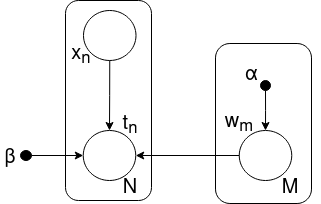
\includegraphics[scale=0.5]{images/problem_8.5.png}
	\caption{Relevance vector machine graphical model}
	\label{fig:boat1}
\end{figure}

\section*{Problem 8.6}

As we can see, each variable $x_i$ has an effect of multiplying negative term by $(1 - \mu_i)^{x_i}$. If $x_i$ is zero, this factor reduces to 1. But, if $x_i$ is 1, this turns into $(1-\mu_i)$, which is the probability of $x_i$ being zero. The greater this probability is (i.e. the smaller is $\mu_i$) the greater will be the negative factor. So this accounts to the fact that $x_i$ could be 1 because of noise with the probability  $\mu_i - 1$. $\mu_0$ is the probability of $y$ being 1 when all $x_1..x_N$ are zeros. 

\section*{Problem 8.8}

From the statement of the problem we know that $p(a,b,c|d) = p(a|d)p(b,c|d)$, and we need to prove $p(a,b|d) = p(a|d)p(b|d)$.

To prove this, we just integrate over $c$ the known equality: $\int\limits_{c}p(a,b,c|d) = \int\limits_{c}p(a|d)p(b,c|d) = p(a|d)\int\limits_{c}p(b,c|d) = p(a|d)p(b|d)$.

On the other hand, $\int\limits_{c}p(a,b,c|d) = p(a,b|d)$ and so the equality is proven. 

\section*{Problem 8.9}

Let us consider a node describing variable $x$ and its Markov blanket. Let us consider any $y \notin Blanket(x)$ and show that any path from it to $x$ is blocked. The last node on this path before $x$ can be either:
\begin{itemize}
	\item parent of $x$
	\item child of $x$
\end{itemize}

First suppose there is a path from $y$ to $x$ which includes some parent $z$ of $x$ as a last node in the path (except $x$). Such a path is blocked by the corresponding parent because the arrows on this path are head-to-tail or tail-to-tail (because $z$ is a parent of $x$, the arrow goes from $z$ to $x$).

Now let us consider the situation when the path from $y$ to $x$ ends with a child $u$ of $x$. Then we need again to consider two options:
\begin{itemize}
	\item the path enters $u$ via arrow
	\item the path enters $u$ via tail
\end{itemize}

In the first case, the path goes from $v$ to $u$, where $v$ is a co-parent of $x$. It can be seen that $v$ blocks the path because it has a tail-to-tail or tail-to-head connection at $v$.

In the second case, the path has a tail-to-head connection at $u$ and is blocked by $u$.

So, in any case, the path from $y$ to $x$ is blocked.

\section*{Problem 8.10}

The only path from $a$ to $b$ goes through $c$. It enters $c$ head-to-head and so when no variables are observed, this path is blocked by the second condition of D-separation.

When either $c$ or $d$ is observed, this path becomes unblocked, and so $a$ starts to depend on $b$. 

\section*{Problem 8.11}
We have that
 \begin{align}
	P(F,D,G,B) = P(F)P(B)P(G|F,B)P(D|G)
\end{align}

And we will use the following equation, inferred from the bayes' theorem application:
\begin{align}
	P(F|D) = \frac{P(F,D)}{P(D)}
\end{align}

\begin{align}
\begin{split}
P(F=0,D=0,B=0,G=0) = 0.1 * 0.1 * 0.9 * 0.9 = 0.0081\\
P(F=0,D=0,B=0,G=1) = 0.1 * 0.1 * 0.1 * 0.1 = 0.0001\\
P(F=0,D=0,B=1,G=0) = 0.1 * 0.9 * 0.8 * 0.9 = 0.0648\\
P(F=0,D=0,B=1,G=1) = 0.1 * 0.9 * 0.2 * 0.1 = 0.0018
\end{split}
\end{align}

So, $P(F = 0,D = 0) = 0.0748$

\begin{align}
\begin{split}
	P(F=1,D=0,B=0,G=0) = 0.9 * 0.1 * 0.8 * 0.9 = 0.0648\\
	P(F=1,D=0,B=0,G=1) = 0.9 * 0.1 * 0.2 * 0.1 = 0.0018\\
	P(F=1,D=0,B=1,G=0) = 0.9 * 0.9 * 0.2 * 0.9 = 0.1458\\
	P(F=1,D=0,B=1,G=1) = 0.9 * 0.9 * 0.8 * 0.1 = 0.0648
\end{split}
\end{align}

So, $P(F = 1,D = 0) = 0.2772$

\begin{align}
P(F = 0|D=0) = \frac{P(F = 0, D = 0)}{P(D=0)} = \frac{0.0748}{0.0748 + 0.2772} = 0.2125
\end{align}

Now let us suppose we also know, that the battery is flat ($B = 0$):

$P(F = 0,D = 0,B =0) = 0.0082$

And thus we get
\begin{align}
P(F = 0|D=0,B=0) =  \frac{P(F = 0, D = 0, B=0)}{P(D=0,B=0)} = \frac{0.0082}{0.0666 + 0.0082} = 0.1096
\end{align}

So the probability of tank being empty in case we know battery is flat and driver reported the gauge shows empty is indeed lower than the same probability but when we do not know the battery is actually flat. The intuition behind is that if we know the battery is flat, it can be the reason why the gauge shows the tank is empty (whether it is really empty or not), and as driver's report is highly correlated with the gauge readings, we should have less belief in the driver's report results. 

This means that $P(F|D,B) \ne P(F|D)$, so tank emptiness and battery flattness are not independent conditioned on driver's report, while they are independent inconditionally. This shows that conditioning on the decendants ($D$) of the collider ($G$) leads to unblocking the association path in graphical models.
\end{document}